%===================================================================================
% Chapter: Propuesta para la Extracción de Relaciones
%===================================================================================
\chapter{Propuesta para la Extracción de Relaciones}\label{chapter:relations}
\addcontentsline{toc}{chapter}{Extracción de Relaciones}

En este capítulo se hace una descripción de las técnicas empleadas para la resolución de la tarea de Extracción de Relaciones.
Primeramente, se recoge un resumen del análisis de dependencias de una oración, aspecto cardinal en la propuesta realizada.
Luego se describe el modelo de aprendizaje profundo propuesto y sus componentes.


\section{Análisis de Dependencias}\label{sec:parsing}

El conocimiento de la estructura y la sintaxis que subyace en un texto en lenguaje natural puede ser de mucha ayuda en tareas típicas de NLP, incluyendo la Extracción de Relaciones.
Una de las técnicas más comunes para capturar cierta estructura en las oraciones es el análisis sintáctico~(conocido comúnmente por su nombre en inglés: \emph{parsing}).

Se han descrito dos formas esenciales de explicar la estructura de una oración en lenguaje natural: separando la oración en \textbf{constituyentes}~(frases), que se separan a su vez en constituyentes más pequeños; o estableciendo conexiones entre las palabras individuales~\cite{covington2001fundamental}.
El significado de estas dos variantes se ilustra en las figuras \ref{fig:dep_const} y \ref{fig:dep_links} respectivamente.

\begin{figure}[h!]
	\centering
	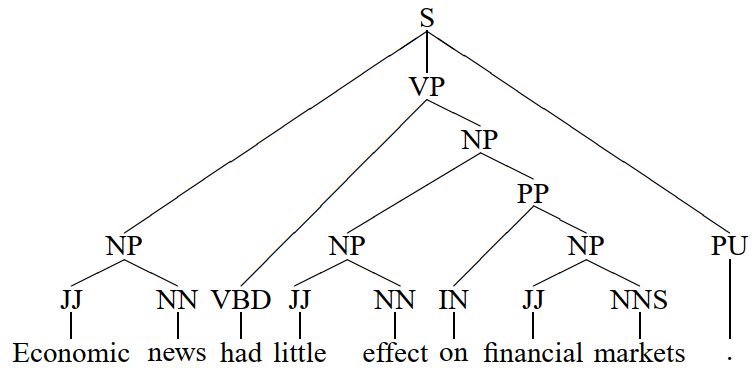
\includegraphics[width=0.8\linewidth]{Graphics/dep_const.png}
	\caption{Estructura constituyente para una oración en idioma inglés del \emph{Penn Treebank}.}\label{fig:dep_const}
\end{figure}

\begin{figure}[h!]
	\centering
	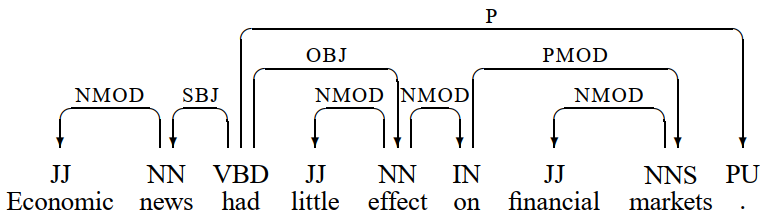
\includegraphics[width=0.8\linewidth]{Graphics/dep_links.png}
	\caption{Estructura de dependencias para una oración en idioma inglés del \emph{Penn Treebank}.}\label{fig:dep_links}
\end{figure}

La representación constituyente del lenguaje data de varios años atrás, y ha sido explotada tanto por los científicos de la computación como por lingüistas, en aras de obtener buenas representaciones del lenguaje natural.
Sin embargo, la comunidad científica ha mostrado un creciente interés en los últimos años en las estructuras de dependencias como una alternativa a esta representación.

La noción fundamental de \textbf{dependencia} está basada en la idea de que la estructura sintáctica de una oración está conformada por un conjunto de relaciones binarias asimétricas entre las palabras de dicha oración~\cite{nivre2005dependency}.
Siempre que se establece una relación entre dos palabras, a una de ellas se le denomina \textbf{cabecera} y a la otra \textbf{dependiente}.
A continuación se listan algunos criterios que han sido propuestos para identificar una relación sintáctica entre una cabecera $H$ y un dependiente $D$, en una construcción sintáctica $C$~\cite{zwicky1985heads, richard1990english}:

\begin{enumerate}
	\item $H$ determina la categoría sintáctica de $C$, y muchas veces puede sustituir a $C$.
	
	\item $H$ determina la categoría semántica de $C$, mientras que $D$ aporta especificidad.
	
	\item $H$ es obligatoria, mientra que $D$ es opcional.
	
	\item $H$ selecciona a $D$, y determina si puede o no ser opcional.
	
	\item La forma de $D$ depende de $H$.
	
	\item La posición de $D$ en la oración se especifica con respecto a $H$.
\end{enumerate}

Estas reglas no son absolutas y contienen un mezcla de criterios variados, algunos sintácticos, otros semánticos.
No existe en la literatura una noción coherente de dependencia que se corresponda con todos los distintos criterios~\cite{nivre2005dependency}.


\subsection{Grafo de dependencias}

Si se considera cada dependencia como un arco dirigido que tiene como origen a la cabecera y como destino al dependiente, la estructura de dependencias de la oración conforma un grafo dirigido $G$ cuyos nodos son los elementos léxicos del lenguaje~(\emph{tokens}).
Además, el grafo subyacente de $G$ debe ser conexo, para que cada nodo esté relacionado con, al menos, otro nodo.

A esta caracterización se le imponen usualmente más restricciones.
Dos de las más utilizadas en las distintas formalizaciones de gramáticas basadas en dependencias~(o simplemente, gramáticas de dependencias), son: la suposición de que cada nodo del grafo tiene \emph{indegree} $\leq 1$; y la no existencia de ciclos.
Estas suposiciones, junto a la consideración de conectividad, implican que este grafo sea un árbol dirigido con una sola raíz la cual no depende de ninguna otra palabra.
Esto último queda ilustrado en la figura \ref{fig:dep_tree}.
A esta estructura se le denomina \textbf{árbol de dependencias}.

\begin{figure}[h!]
	\centering
	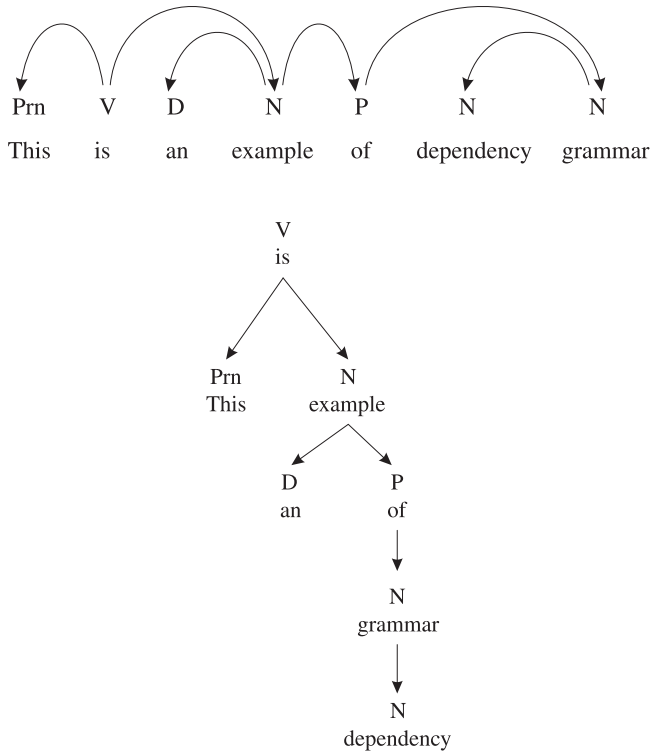
\includegraphics[width=0.7\linewidth]{Graphics/dep_tree.png}
	\caption{Estructura de dependencias para una oración en idioma inglés y árbol de dependencias.}\label{fig:dep_tree}
\end{figure}

Existen varias restricciones adicionales que se definen sobre estas estructuras y que son más debatidas.
Una de las más conocidas es la restricción de \textbf{proyectividad}~\cite{hays1964dependency,lecerf1960programme,marcus1965notion}.
Un grafo de dependencias satisface la restricción de proyectividad con respecto a un orden linear particular de los nodos si, por cada arco $h \rightarrow d$ y un nodo $w$, $w$ ocurre entre $h$ y $d$ en el orden lineal solo si $w$ está \textbf{dominado} por $h$~\footnote{La relación \textbf{dominar} es la clausura reflexiva y transitiva de la relación de dependencia definida por los arcos}. 

\section{Modelo de Aprendizaje Profundo}\label{sec:model}

El modelo de aprendizaje profundo propuesto se apoya en el uso de redes neuronales recurrentes sobre estructuras derivadas del árbol de dependencias de la oración de entrada y las entidades señaladas, para obtener una representación de la hipotética relación existente entre ellas.

\subsection{Hipótesis del Camino en el Árbol de Dependencias}

Como fue explicado en el capítulo~\ref{chapter:information_extraction}, la información más completa para resolver el problema de la Extracción de Relaciones se encuentra en la oración íntegra. Sin embargo, se maneja por muchos autores la suposición de que el árbol de dependencias de la oración de entrada condensa la información vital, a la vez que desecha otras fuentes de desinformación.

El hecho de que las entidades entre las cuales se quiere determinar la existencia de una relación estén formadas por múltiples palabras, constituye un problema para la configuración de algoritmo de aprendizaje profundo.
Es factible, en términos de implementación, concebir una configuración que permita establecer la existencia de relaciones entre dos palabras o \textit{tokens} de la oración.
Pero si las entidades están formadas por múltiples palabras, un aspecto cardinal de la implementación consiste en definir qué palabra va a \textit{representar} a la entidad a la hora de determinar las relaciones en las que participa.
Con este fin se han explorado diversos criterios en la literatura.
Se debate el uso de la última palabra de la entidad en algunos casos; en otros, de la primera.

De manera general, de acuerdo a observaciones realizadas sobre el conjunto de datos estudiado, las entidades señaladas constituyen unidades sintácticas coherentes; llegando a ser sintagmas nominales completos, en varios ejemplos.
Como fue abordado, uno de los criterios que determina la existencia de una dependencia con una cabecera \textit{H} en una construcción sintáctica \textit{C}, es que \textit{H} puede sustituir sintácticamente a \textit{C}.
Incluso, \textit{H} puede determinar semánticamente a \textit{C}.
Por otro lado, las entidades formadas por múltiples palabras suelen ocurrir de manera total en un subárbol del árbol de dependencias, que tiene como raíz una de las palabras de la entidad.
Este hecho fue explorado en el conjunto de datos estudiado, y se cumple en la amplia mayoría de los casos, exceptuándose muy pocos ejemplos.
Dicho subárbol correspondiente a una entidad \textit{e} lo definimos como \textbf{subárbol relevante a \textit{e}}, y lo denotamos como $S_e$.
A la raíz de dicho subárbol la denominamos \textbf{núcleo de la entidad $e$}, y se denota como $n_e$.

Otra definición importante, citada repetidamente en la literatura para resolver este problema es el \textbf{camino en el árbol de dependencias} entre dos \textit{tokens} $t_1,t_2$.
Esta definición es intuitiva, y denota a la secuencia de \textit{tokens} que ocurren en el camino que va desde $t_1$ hasta $t_2$.
Dicho camino será denotado como $C(t_1,t_2)$.

La figura \ref{fig:dep_tree_ex} ilustra las definiciones anteriores.

\begin{figure}[h!]
	\centering
	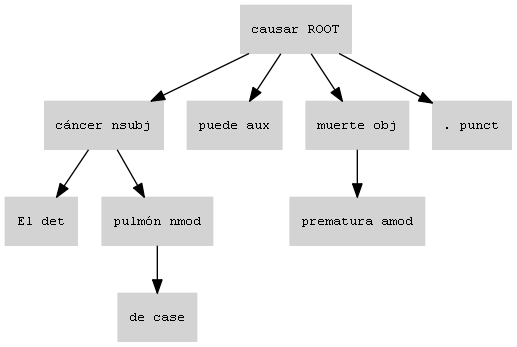
\includegraphics[width=0.7\linewidth]{Graphics/dep_tree_ex.png}
	\caption{Árbol de dependencias de la oración: \textbf{El cáncer de pulmón puede causar muerte prematura}. Se establece la relación \textbf{entails} entre las entidades \textbf{cáncer de pulmón}($e_1$) y \textbf{muerte}($e_2$). Aparecen señalados $S_{e_1}$, $S_{e_2}$, así como $C(n_{e_1}, n_{e_2})$.}\label{fig:dep_tree_ex}
\end{figure}

En la selección del modelo propuesto se consideran dos hipótesis fundamentales a la hora de establecer la existencia de una relación entre el par de entidades $\langle e_1,e_2 \rangle$, las cuales se comprobaron de manera experimental, como será descrito en el capítulo \ref{chapter:experiments}:

\begin{enumerate}
	\item $S_{e_1}$ y $S_{e_2}$ condensan información útil sobre las respectivas entidades, a la vez que deshechan fuentes de desinformación.
	
	\item $C(n_{e_1}, n_{e_2})$ condensa información útil para determinar una posible relación entre $e_1$ y $e_2$, a la vez que deshecha fuentes de desinformación.
\end{enumerate}


\subsection{Red Neuronal}

La configuración de red definida, pretende determinar la existencia de una relación entre las entidades $e_1$ y $e_2$ en el contexto de una oración dada. Para ello codifica la información contenida en los subárboles relevantes a $e_1$ y $e_2$~(denotados $S_{e_1}$ y $S_{e_2}$, respectivamente), así como en el camino en el árbol de dependencias entre los núcleos de $e_1$ y de $e_2$~(denotado $C(n_{e_1}, n_{e_2})$).

Tanto $S_{e_1}$, $S_{e_2}$ como $C(n_{e_1}, n_{e_2})$, son estructuras formadas por palabras de la oración de entrada. Para representar las palabras de la oración en cada una de estas estructuras, se utiliza un vector que se obtiene a partir de la concatenación de \textit{embeddings} provenientes de distintas fuentes de información:

\begin{description}
	\item[\textit{Embedding} Contextual:] Se utilizan \textit{embeddings} contextuales preentrenados, obtenidos a partir del modelo BERT.
	
	\item[\textit{Embedding} de Palabras:] Se utilizan \textit{embeddings} preentrenados en un corpus construido a partir de artículos de Wikipedia con contenido médico.
	
	\item[Caracteres:] Se utilizan \textit{embeddings} obtenidos mediante una CNN sobre los caracteres de la palabra.
	
	\item[POST-tag y Dependencia:] Se utiliza un \textit{embedding} de la etiqueta de POS-tag de la palabra y la dependencia de la misma con su ancestro en el árbol de dependencias de la oración.
	
	\item[Etiqueta BMEWO-V y Tipo de la entidad:] Se añaden \textit{embeddings} con información relativa a la entidad a la que pertenece la palabra en cuestión.
	En este caso la etiqueta correspondiente en el sistema BMEWO-V así como el tipo de la entidad.
	
\end{description}

A partir de esta representación distruibuida de las estructuras $S_{e_1}$, $S_{e_2}$ y $C(n_{e_1}, n_{e_2})$, se obtiene una representación de la oración y las entidades señaladas.
Primeramente, una capa BiLSTM transforma la representación de cada palabra de la secuencia $C(n_{e_1}, n_{e_2})$, para incluir información contextual de las palabras anteriores y posteriores de cada posición.

\begin{equation*}
	P = BiLSTM(C(n_{e_1}, n_{e_2}))
\end{equation*}

Luego, la capa LSTM apilada enfatiza la direccionalidad de la relación, procesando la secuencia $P$ solamente en el sentido que va desde el origen hacia el destino de la misma, y obtiene un vector $p$ que codifica la información contenida en $C(n_{e_1}, n_{e_2})$.

\begin{equation*}
	p = LSTM(P)
\end{equation*}

Entre tanto, una capa recurrente se aplica sobre $S_{e_1}$ y $S_{e_2}$ de manera independiente~\footnote{Las representaciones de $S_{e_1}$ y $S_{e_2}$ se obtienen de manera independiente, pero utilizando el mismo conjunto de parámetros.}.
En este caso se utiliza una red Tree-LSTM, en su variante \textit{Child Sum}~\cite{tai2015improved}.

\begin{equation*}
	t_{e_1} = TreeLSTM(S_{e_1})
\end{equation*}


\begin{equation*}
	t_{e_2} = TreeLSTM(S_{e_2})
\end{equation*}


Una red Tree-LSTM es una generalización de una red LSTM, que permite procesar de manera recurrente estructuras de vectores que se organicen en forma de grafos dirigidos y acíclicos~(como los árboles, por ejemplo).

Una celda Tree-LSTM en el momento $t$, al igual que su homólogo lineal, se define como una colección de vectores en $\mathbb{R}^d$, siendo $d$ la dimensión oculta de dicha celda.
Estos vectores son: una compuerta de entrada $i_t$, una compuerta de olvido $f_t$, una compuerta de salida $o_t$, una celda de memoria $c_t$ y un estado oculto $h_t$. Siendo $C(j)$ la secuencia de hijos de el nodo $j$, las ecuaciones de transición de una celda Tree-LSTM se muestran a continuación:

\begin{equation*}
	\overline{h}_j = \sum_{k\in C(j)} h_k
\end{equation*}

\begin{equation*}
i_j = \sigma(W^{(i)}x_j + U^{(i)}\overline{h}_j + b(i))
\end{equation*}

\begin{equation*}
f_{jk} = \sigma(W^{(f)}x_j + U^{(f)}h_k + b(f))
\end{equation*}

\begin{equation*}
o_j = \sigma(W^{(o)}x_j + U^{(o)}\overline{h}_j + b(o))
\end{equation*}

\begin{equation*}
u_j = tanh(W^{(u)}x_j + U^{(u)}\overline{h}_j + b(u))
\end{equation*}

\begin{equation*}
c_j = i_j \odot u_j + \sum_{k\in C(j)} f_{jk} \odot c_k
\end{equation*}

\begin{equation*}
h_j = o_j \odot tanh(c_j)
\end{equation*}

Nótese que la diferencia con respecto a las redes LSTM radica en que, como se tienen varios momentos inmediatos anteriores al momento $t$, se considera la suma de todos los respectivos estados ocultos. La figura \ref{fig:lstm_cmp} ilustra las diferencias entre ambas.

\begin{figure}[h!]
	\centering
	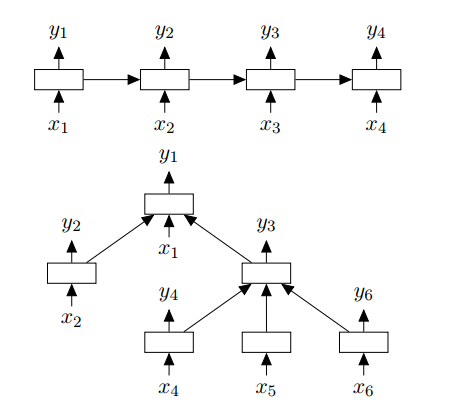
\includegraphics[width=0.7\linewidth]{Graphics/lstm_cmp.png}
	\caption{\textbf{Arriba}: LSTM tradicional o de cadena. \textbf{Abajo}: Tree-LSTM~\cite{tai2015improved}.}\label{fig:lstm_cmp}
\end{figure}

Loa vectores obtenidos a partir de la secuencia de entrada y las entidades señaladas se concatenan para formar la representación de la hipotética relación.

\begin{equation*}
	r = [t_{e_1}; t_{e_2}; p]
\end{equation*}

La salida $x$ se obtiene a partir de aplicar la función sigmoide a una transformación linear de dicho vector.

\begin{equation*}
	x = \sigma(W^{(x)}r + b^{(x)})
\end{equation*}

La matriz $W^{(x)}$ tiene dimensiones $k \times l$, donde $l = |t_{e_1}| + |t_{e_2}| + |p|$ y $k$ es el número de relaciones semánticas diferentes que se definen.

De acuerdo al vector de salida $x$, se predice la existencia de una relación si su valor máximo excede un umbral prefijado que se introduce como un hiperparámetro adicional. De ser así, se predice la existencia solamente de la relación dada por $argmax(x)$.
	
Nótese como, a diferencia de las arquitecturas típicas, esta configuración permite prescindir de la relación ficticia \textit{none}.

La figura \ref{fig:rel_model} ilustra la arquitectura descrita.

\begin{figure}[h!]
	\centering
	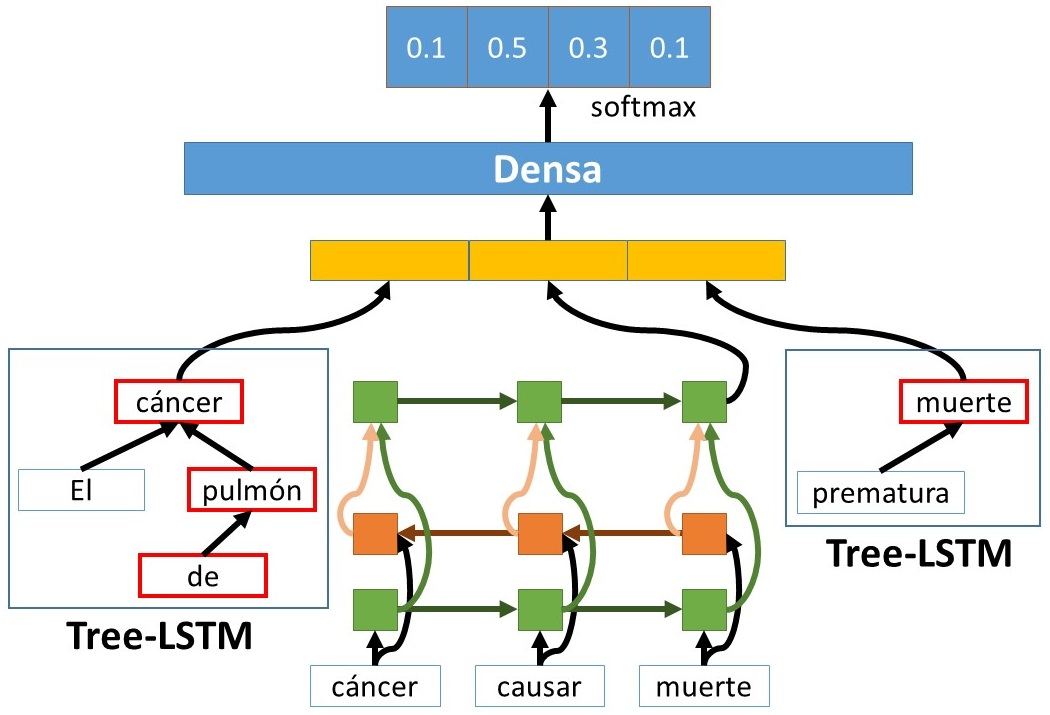
\includegraphics[width=1\linewidth]{Graphics/rel_model_class.jpg}
	\caption{Arquitectura de red utilizada. La oración de entrada es \textbf{El cáncer de pulmón puede causar muerte prematura} Y las entidades en cuestión son \textbf{cáncer de pulmón} y \textbf{muerte}.}\label{fig:rel_model}
\end{figure}

\section{Entrenamiento}

Debido a que la salida correspondiente a cada relación es independiente de las otras, el modelo se entrena para minimizar una función de entropía binaria.
Siendo $k$ el número de relaciones definidas, la función de pérdida entre la salida del modelo $x$ y un vector binario $y$ objetivo, se define como:

\begin{equation*}
	\ell(x, y) = \frac{1}{k}\sum_{1\leq i\leq k}{\left[ y_i \cdot \log x_i + (1 - y_i) \cdot \log (1 - x_i) \right]}
\end{equation*}

Como fue explicado, la salida del modelo no expresa directamente la existencia de una relación ficticia que contemple el caso de la no existencia de relación entre el par de entidades de entrada.
Para que el modelo sea capaz de reconocer estos casos, se introduce una estrategia de muestreo negativo durante el entrenamiento, donde el vector objetivo es el vector nulo.
Dicho muestreo no se realiza utilizando como entrada pares de palabras aleatorios, sino núcleos de entidades existentes en la oración entre las cuales no existe una relación.
En el capítulo \ref{chapter:experiments} se describirán experimentos realizados con distintas estrategias de muestreo negativo utilizadas.

%===================================================================================